\documentclass{article}

\usepackage[utf8]{inputenc}
%\usepackage[english]{babel}
%\usepackage[]{algorithm2e}
\usepackage{verbatim}
\usepackage{program}
\usepackage{listings}
\usepackage{graphicx}
%\usepackage[]{algorithm2e}
\usepackage{titlesec}
\usepackage{hyperref}
\graphicspath{ {images/} }

\titleclass{\subsubsubsection}{straight}[\subsection]

\newcounter{subsubsubsection}[subsubsection]
\renewcommand\thesubsubsubsection{\thesubsubsection.\arabic{subsubsubsection}}
\renewcommand\theparagraph{\thesubsubsubsection.\arabic{paragraph}} % optional; useful if paragraphs are to be numbered

\titleformat{\subsubsubsection}
  {\normalfont\normalsize\bfseries}{\thesubsubsubsection}{1em}{}
\titlespacing*{\subsubsubsection}
{0pt}{3.25ex plus 1ex minus .2ex}{1.5ex plus .2ex}

\makeatletter
\renewcommand\paragraph{\@startsection{paragraph}{5}{\z@}%
  {3.25ex \@plus1ex \@minus.2ex}%
  {-1em}%
  {\normalfont\normalsize\bfseries}}
\renewcommand\subparagraph{\@startsection{subparagraph}{6}{\parindent}%
  {3.25ex \@plus1ex \@minus .2ex}%
  {-1em}%
  {\normalfont\normalsize\bfseries}}
\def\toclevel@subsubsubsection{4}
\def\toclevel@paragraph{5}
\def\toclevel@paragraph{6}
\def\l@subsubsubsection{\@dottedtocline{4}{7em}{4em}}
\def\l@paragraph{\@dottedtocline{5}{10em}{5em}}
\def\l@subparagraph{\@dottedtocline{6}{14em}{6em}}
\makeatother

\setcounter{secnumdepth}{4}
\setcounter{tocdepth}{4}


\begin{document}

\title{Parallelos Games\\\
Numerical Analisis Proyect}
\author{
\\\\\\\\\\
 Team:\\\\
  Mateo Hincapi\'e Zapata\\\\
  Mauricio Hoyos Ardila\\\\
  Dillan Alexis Muñet\'on Avendaño\\\\
  Pablo Quijano Jaramillo\\\\
  Marcos David Sierra Gallego\\\\
  Jonathan Stiven Zapata Castaño\\\\\\\\\\
  Teacher:\\\\
  Francisco Jos\'e Correa Zabala\\\\\\\\\\
  Universidad Eafit\\\\
  }
\date{October, 2017}

\maketitle

\newpage

\tableofcontents

\newpage

\section{Introduction}

Technology has become every time more and more necessary in people's lives. Nowadays it has a lot of uses, one of them being the computing application in the mathematics world. Numerical methods  are a tool to help to solve numerical
problems. Sometimes, this problems are really complex and hard to solve by
the human. For this reason, we can say that exists a relation between numerical
methods  and the computing world because the computers can process a lot of data
and solve faster the problems than humans.\\

Even though there are computers that
can process big amount of data, there is another problem. People usually do not take full advantage of the capacity that computers have . Normally, computers have from 4 to 8 processors, and people only use one of them. This is also happening
with numerical methods. We are not using the true capacity of computers to solve numerical problems.\\


\section{Project description}

This project is focused in work with numerical methods using all the capacity that the computer has. With this, we are searching better results about the
converge speed and the most efficient solution that the methods can give us.

\subsection{Methodology}


This Project has been divided in different parts or stages to manage the goal:

\begin{itemize}

\item Reading and understanding of the practice. This component gave us the first idea to start working in parallel.

\item Basic algorithms implementation in parallel. The best way to understand how parallel methods work is practising by doing easy examples about it.

\item Work with the use of matrices in parallel to make better, faster, and more efficient its operations.

\item Implementation of some numerical methods in parallel which we’ve seen in class. In this case, we work with big dimension matrices to solve methods like Gauss or Jacobi.

\item Analysis and testing of the performance of algorithms methods.

\end{itemize}

\subsection{Project Structure}

This project will has the following structure and it contains the following folders:

\begin{itemize}

\item \textbf{Informs:}This folder has the final inform of this project.

\item \textbf{Parallel:}Here, you can find the parallel codes of some numerical methods .

\item \textbf{Serial:}Here, you can find the serial codes of some numerical methods .

\item \textbf{Blocks:} This folder contains the source code of big matrices solution and its generator.

\item \textbf{Added Values:} source code of methods that we have seen in class.


\end{itemize}
 
This project is available in GitHub on the link https://github.com/jonyzp/parallelGames

\subsection{Compilation mode and execution}
In the moment that we’re going to run a program in C++, first is necessary compile the program. But the compilation with our programs is different, because we are using openMP,  which is the library that we use to programming in parallel. then, the compilation change a little.
We’ll compile the next form. g++ -o nameOut -fopenmp [nameProgram].cpp, when the instruction fopenmp indicate that the program will work in parallel, have zones in parallel and it use the library openMP.\\

\subsubsection{Execution with openMP}
When we execute the program then to compile, the program need execution permissions, in this case es similar that execute a normal program of C++. The executable that the compilation let me, we’ll execute of the next form (in Linux). ./nameProgram. 
With the last instruction, the program show us its result in the terminal.\\


\subsubsection{Excecution of matrix generator and methods}
In this part, we'll explain how to compile and execute some method from this section, with different matrix of different sizes.\\\\
First, generate a matrix of our preference as follows:
\begin{itemize}
\item Compile java file `generator.java' with the comand: `javac generator.java'.
\item Execute `generator.exe' specifying the filename, for example, if you want a matrix of size 1000x1000, so you execute this command: \\
`java generator $>$ matrixName.txt', follows by the number `1000'.
\item Then, you have a 1000x1000 matrix in the file `matrixName.txt'.
\end{itemize}
Second, compile the method as follows:
\begin{itemize}
\item Use the comand: `g++ fileNameMethod.cpp -o fileNameMethod' to compile.
\item Then, you have an executable file, execute this with the command: \\
`./fileNameMethod' and next give it where is the matrix to be processed and the file for write the solution.
\item At this point, you must have a file with the solution.
\end{itemize}

All this instructions about compilation and execution have to be done for each method you can run.


\subsection{Gaussian Elimination}

\subsubsection{Description:}

In this section, we are going to show how to parallelize the gaussian elimination method, which is one of the most simple methods to solve equations systems, the simple gaussian elimination, in spite of that this algorithm is not very efficient in its serial form, it has the advantage that is highly parallelizable. For example, you can do an aperation which is the same for many rows at the time, sending one thread to each line and do this efficiently. Then, when it finish, we have to apply the backward substitution to obtain the solution of the system. In order to improve the speed of the execution, we are going to try with different amount of threads and matrix.

\subsubsection{Code:}

\subsubsubsection{Parallel}

\begin{lstlisting}[language=C]

void gaussElimination(){
  for ( k= 0; k < n-1; ++k)
  {
    #pragma omp parallel for private( i,j,multi)
    for ( i = k+1; i < n; ++i)
    {
      multi= m[i][k]/m[k][k];
      m[i][k] =0;
      for (j = k+1; j< n+1; ++j)
      {
        m[i][j] = double(m[i][j]- multi* m[k][j]);
      }
    }
  }
}

\end{lstlisting}

\subsubsubsection{Serial}

\begin{lstlisting}[language=C]

void gaussElimination(){
  for ( k= 0; k < n-1; ++k)
  {
    for ( i = k+1; i < n; ++i)
    {
      multi= m[i][k]/m[k][k];
      m[i][k] =0;
      for (int j = k+1; j< n+1; ++j)
      {
        m[i][j] = double(m[i][j]- multi* m[k][j]);
      }
    }
  }
}
\end{lstlisting}

\subsubsection{Analysis of the method:}
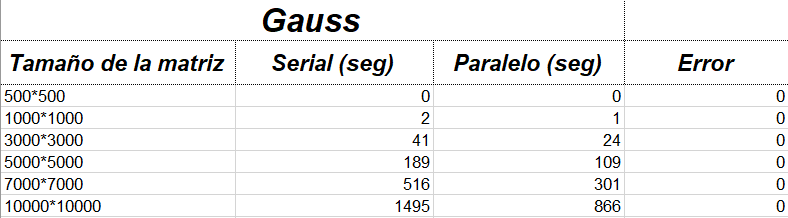
\includegraphics[width=\linewidth]{./images/gauss.PNG}\\

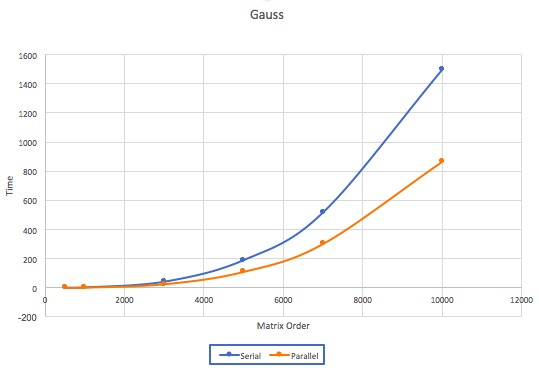
\includegraphics[width=\linewidth]{./images/gg.jpeg}\\


\subsection{LU Factorization}

\subsubsection{LU}

\subsubsubsection{Description}

In many applications where linear systems appear, one needs to solve Ax = b for many different vectors b.
For instance, a structure must be tested under several different loads, not just one. As in the example of a
truss (9.2), the loading in such a problem is usually represented by the vector b. Gaussian elimination with
pivoting is the most efficient and accurate way to solve a linear system. Most of the work in this method is
spent on the matrix A itself. If we need to solve several different systems with the same A, and A is big,
then we would like to avoid repeating the steps of Gaussian elimination on A for every different b. This can
be accomplished by the LU decomposition, which in effect records the steps of Gaussian elimination.



\subsubsubsection{Code}

\begin{lstlisting}[language=C]


void gaussianElimination(int n){
	
	for(k=0; k<n; ++k){
		L[k][k]=1;
        #pragma omp parallel for private( i,j,multiplier) 
		for(i=k+1; i<n; ++i){
			multiplier = U[i][k]/U[k][k];
			L[i][k]=multiplier;
			for(j=k; j<n; ++j){
				U[i][j] = U[i][j] - multiplier*U[k][j];
			}
		}
	}
}

\end{lstlisting}


\subsubsubsection{Analysis of the method:}

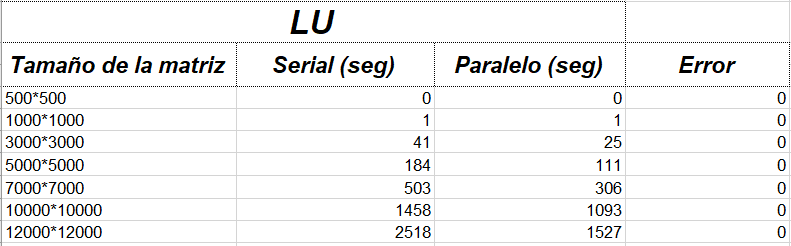
\includegraphics[width=\linewidth]{./images/lu.PNG}\\
In this graphic we can see the result and the comparison between serial form and parallel form.

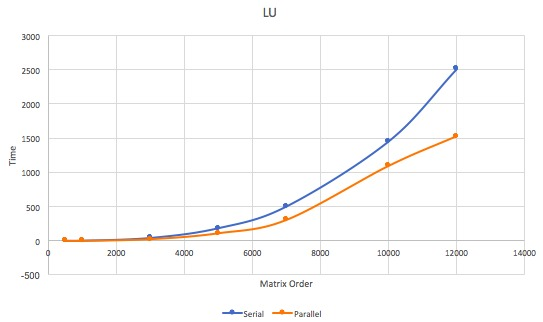
\includegraphics[width=\linewidth]{./images/glu.jpeg}\\


\subsubsection{LU Cholesky}

\subsubsubsection{Description}

Cholesky decomposition is a special version of LU decomposition tailored to handle symmetric
matrices more efficiently.
For a symmetric matrix A, by definition, aij = aji. LU decomposition is not efficient enough
for symmetric matrices. The computational load can be halved using Cholesky decomposition.



\subsubsubsection{Code}

\begin{lstlisting}[language=C]

void cholesky(int n){
    double suma1,suma2,suma3;
    
    for(k=0;k<n;++k){
        suma1=0;
        #pragma omp parallel for private( m) shared(suma1,k,L,U)
        for(m=0;m<k;++m){
            suma1+=L[k][m]*U[m][k];
        }
        L[k][k]=sqrt(A[k][k]-suma1);
        U[k][k]=L[k][k];
        #pragma omp parallel for private(i,suma2,p) shared(L,U,k)
        for(i=k;i<n;++i){
            suma2=0;
            for(p=0;p<k;++p){
                suma2+=L[i][p]*U[p][k];
            }
            L[i][k]=(A[i][k]-suma2)/(double)U[k][k];
        }
        #pragma omp parallel for private( j,suma3,h) shared(k,L,U)
        for( j=k+1;j<n;++j){
            suma3=0;
            //#pragma omp parallel for default(shared) reduction(+:suma3)
            for(h=0;h<k;++h){
                suma3+=L[k][h]*U[h][j];
            }
            U[k][j]=(A[k][j]-suma3)/(double)L[k][k];
         
        }

    }
}

\end{lstlisting}


\subsubsubsection{Analysis of the method:}

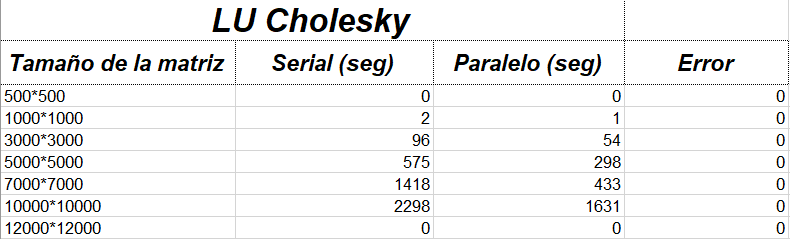
\includegraphics[width=\linewidth]{./images/cholesky.PNG}\\
In this graphic we can see the result and the comparison between serial form and parallel form.

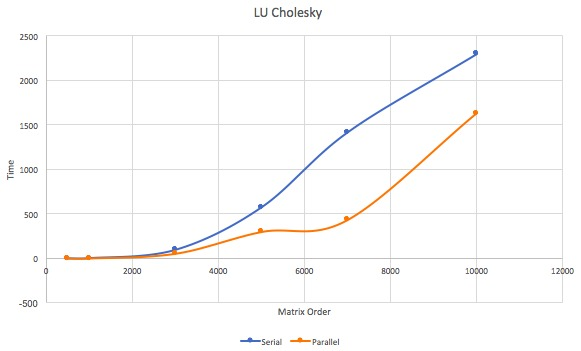
\includegraphics[width=\linewidth]{./images/gluch.jpeg}\\


\subsubsection{LU Crout}

\subsubsubsection{Description}

The Crout matrix decomposition is an LU decomposition which decomposes a matrix into a lower triangular matrix (L), an upper triangular matrix (U) and, although not always needed, a permutation matrix (P). It was developed by Prescott Durand Crout. [1]
The Crout matrix decomposition algorithm differs slightly from the Doolittle method. Doolittle's method returns a unit lower triangular matrix and an upper triangular matrix, while the Crout method returns a lower triangular matrix and a unit upper triangular matrix.
So, if a matrix decomposition of a matrix A is such that:
A = LDU
being L a unit lower triangular matrix, D a diagonal matrix and U a unit upper triangular matrix, then Doolittle's method produces
A = L(DU)
and Crout's method produces
A = (LD)U.
being L a lower triangular matrix, D a diagonal matrix and U a normalised upper triangular matrix



\subsubsubsection{Code}

\begin{lstlisting}[language=C]

void crout(int n){
    double suma1,suma2,suma3;
    int m,i,p,j,h;
    for(int k=0;k<n;++k){
        suma1=0;
        #pragma omp parallel for private( m) shared(suma1,k,L,U)
        for(m=0;m<k;++m){
            suma1+=L[k][m]*U[m][k];
        }
        L[k][k]=A[k][k]-suma1;
        U[k][k]=1;
        #pragma omp parallel for private(i,suma2,p) shared(L,U,k)
        for(i=k;i<n;++i){
            suma2=0;
            for(p=0;p<k;++p){
                suma2+=L[i][p]*U[p][k];
            }
            L[i][k]=(A[i][k]-suma2);
        }
        #pragma omp parallel for private( j,suma3,h) shared(k,L,U)
        for(j=k+1;j<n;++j){
            suma3=0;
            for(h=0;h<k;++h){
                suma3+=L[k][h]*U[h][j];
            }
            U[k][j]=(A[k][j]-suma3)/L[k][k];
         
        }
    }
}

\end{lstlisting}

\subsubsubsection{Analysis of the method:}

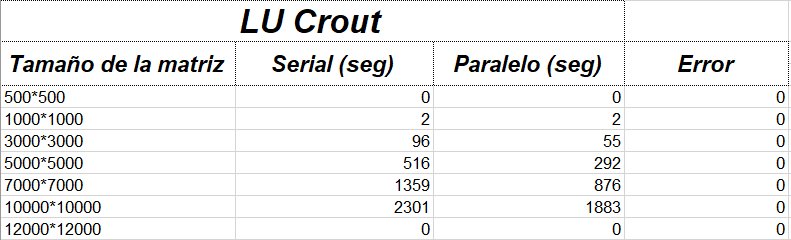
\includegraphics[width=\linewidth]{./images/crout.PNG}\\
In this graphic we can see the result and the comparison between serial form and parallel form.


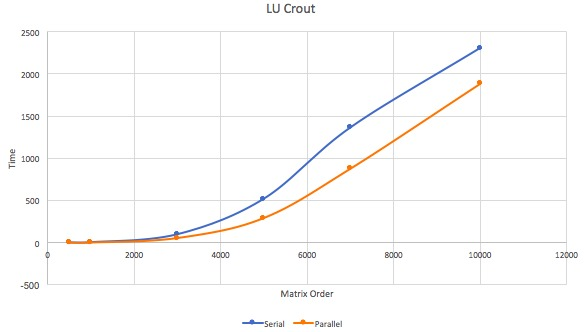
\includegraphics[width=\linewidth]{./images/glucr.jpeg}\\


\subsubsection{LU Dolittle}

\subsubsubsection{Description}

we can factor a square nxn matrix into an LU decomposition, A=LU (where L is an nxn lower triangular matrix whose main diagonal consists of 1's and where U is an nxn upper triangular matrix) using Doolittle's method. Doolittle's method provides an alternative way to factor A into an LU decomposition without going through the hassle of Gaussian Elimination.

Recall that for a general nxn matrix A, we assume that an LU decomposition exists, and write the form of L and U explicitly. We then systematically solve for the entries in in L and U from the equations that result from the multiplications necessary for A=LU.

\subsubsubsection{Code}

\begin{lstlisting}[language=C]

void doolittle (int n){
    double suma1,suma2,suma3;
    int m,i,p,j,h;
    for(int k=0;k<n;++k){
        suma1=0;
        #pragma omp parallel for private( m) shared(suma1,k,L,U)
        for(m=0;m<k;++m){
            suma1+=L[k][m]*U[m][k];
        }
        U[k][k]=A[k][k]-suma1;
        L[k][k]=1;
        #pragma omp parallel for private(i,suma2,p) shared(L,U,k)
        for(i=k;i<n;++i){
            suma2=0;
            for(p=0;p<k;++p){
                suma2+=L[i][p]*U[p][k];
            }
            L[i][k]=(A[i][k]-suma2)/U[k][k];
        }
        #pragma omp parallel for private( j,suma3,h) shared(k,L,U)
        for(j=k+1;j<n;++j){
            suma3=0;
            for(h=0;h<k;++h){
                suma3+=L[k][h]*U[h][j];
            }
            U[k][j]=(A[k][j]-suma3);
         
        }
    }
}

\end{lstlisting}




\subsubsubsection{Analysis of the method:}

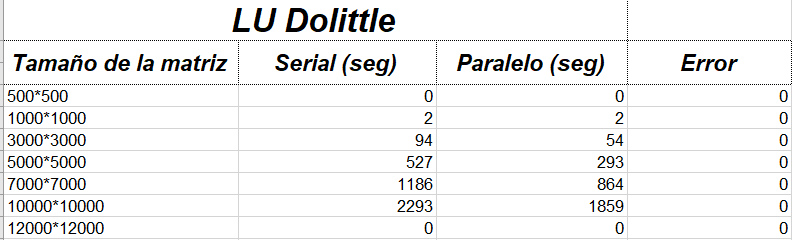
\includegraphics[width=\linewidth]{./images/dolittle.PNG}\\
In this graphic we can see the result and the comparison between serial form and parallel form.


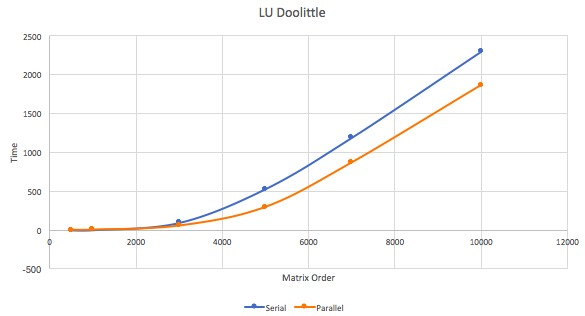
\includegraphics[width=\linewidth]{./images/glud.jpeg}\\


\subsection{Jacobi}

\subsubsection{Description:}
Jacobi is a method to solve linear equations of the form Ax=b. It belongs to the open iterative methods group. its name comes from the German mathematician Carl Gustav Jakob Jacobi.\\

It consists in building a convergent succession defined iteratively. if the algorithm stops after a finite number of steps, it has found an approximation to the values of X of the solution of the problem.\\

The solution is built decomposing the system equation matrix A into:
A = D + L + U where A is the system matrix, D a diagonal matrix, L a lower
triangular matrix and U an upper triangular matrix.
from Ax=b follows:
\begin{center}
  \[Dx + (L + U)x = b\]
\end{center}
after:
\begin{center}
  \[Dx = b – (L + U)x\]
  \[x = D^{-1}[b-(L+U)x]\]
\end{center}
if for each i, $aii \neq  0.$ by iterative rule, the definition of Jacobi can be
expressed as:
\begin{center}
  \[x(k+1) = D-1 [b-(L + U)x(k)]\]
\end{center}
where k is the iterations counter and finally:
\begin{center}
  \[x_{i}^{k+1} = \frac{1}{a_{ii}}*(b_{i}-\sum_{j\neq i}a_{ij}*k_{j}^{k}) , i=1,2,3...\]
\end{center}
For calculate Xi we need all elements in vector X except Xi. This is the most
difference between the methods Jacobi and Gauss-Seidel. The amount of storage
that is required as minimum is two vectors of dimension n.\\

Parallelism in this method is applied in some multiplications that method
requires, we can improve the performance and speed of the method adding this
operations in parallel (sum and multiplication), those are described above.

\subsubsection{Code}

\begin{lstlisting}[language=C]


double newJacobi(int matrixSize){
    double suma, disp,var, aii;
    int i,j;
    disp = 0;
    #pragma omp parallel for shared(xValues, 
    xNewValues, matrix, matrixSize, disp) private(i, j, var, suma, aii)
    for (i = 0; i < matrixSize;++i){
        suma = 0;
        for (j = 0; j < matrixSize;++j){
            var = matrix[i][j];
            if (i!=j)
                suma += var*xValues[j];
            else
                aii = var;
        }
        var = matrix[i][matrixSize];
        xNewValues[i] = (var - suma)/aii;
        disp = max(disp, abs(xNewValues[i]- xValues[i]));
    }
    return disp;
}

bool jacobi(long long matrixSize, double tol, long long niter){
    double disp = tol+1;
    int cont = 0;

    while (disp > tol && cont < niter){
        for (int i = 0; i < matrixSize; ++i){
            xValues[i] = xNewValues[i];
        }
        disp = newJacobi(matrixSize);
        cont++;
    }

    if (disp <= tol)
        return true;
    return false;
}


}


\end{lstlisting}


\subsubsection{Analysis of the method:}


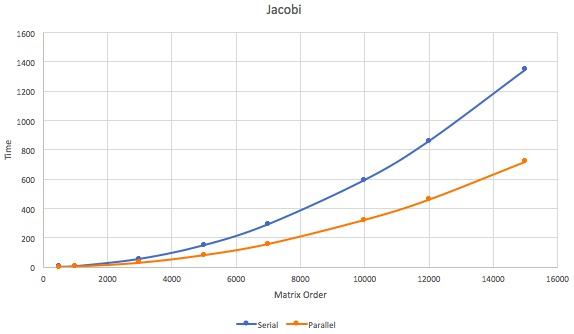
\includegraphics[width=\linewidth]{./images/gj.jpeg}\\

In order to analyse the speed of the method we did some tests with different matrix. So, in the following graphic we can see the performance of jacobi in parallel.

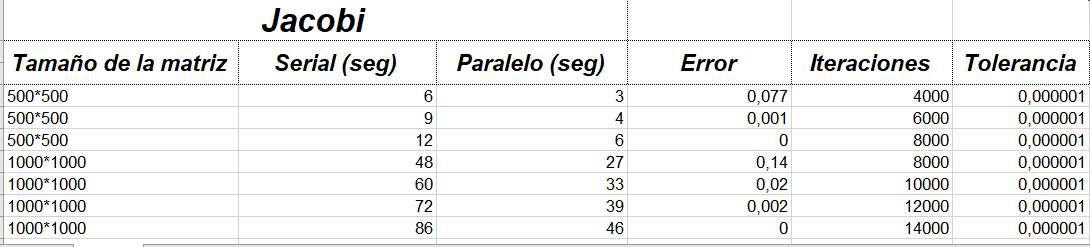
\includegraphics[width=\linewidth]{./images/jacobi.PNG}\\

We can observe that the method increase too much its time of execution when we augment the size of the matrix. Later, we are going to compare this one with another methods, analysing their caracteristics.


\subsection{Gauss Seidel}

\subsubsection{Description:}
 the Gauss–Seidel method is an iterative method used to solve a linear system of equations. It is named after the German mathematicians Carl Friedrich Gauss and Philipp Ludwig von Seidel, and is similar to the Jacobi method. Though it can be applied to any matrix with non-zero elements on the diagonals, convergence is only guaranteed if the matrix is either diagonally dominant, or symmetric and positive definite.

\subsubsection{Code:}

\begin{lstlisting}[language=C]
  double sIteration(int mSize){
    double suma, disp,var, aii, newXValue;
    disp = 0;
    for (int i = 0; i < mSize;++i){
        suma = 0;
        for (int j = 0; j < mSize;++j){
            var = matrix[i][j];
            if (i!=j)
                suma += var*independents[j];
            else
                aii = var;
        }

        var = matrix[i][mSize];
        newXValue =  (var - suma)/aii;
        disp = max(disp, abs(newXValue - independents[i]));
        independents[i] = newXValue;
    }
    return disp;
}

bool gaussS(long long mSize, double tol, long long niter){
    double disp = tol+1;
    int cont = 0;

    while (disp > tol && cont < niter){
        disp = sIteration(mSize);
        cont++;
    }

    if (disp <= tol)
        return true;
    return false;
}

\end{lstlisting}

\subsubsection{Analysis of the method:}


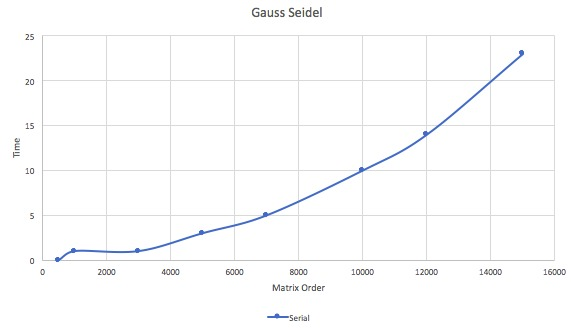
\includegraphics[width=\linewidth]{./images/gs.jpeg}\\

\subsection{Blocks}

In this section of the project, we are going to work with matrices of big dimensions. The structure of this part it's going to contain two differents ways to use the big matrices and two differents iteratives methods, Jacobi and Gauss-Seidel. Both iterative methods are going to work with the two ways of blocks. The first method block consist in read the whole line of the big matrix. The second method block will read a big matrix line divided in two. Also, Jacobi method is working in parallel. In the other side, Gauss-Seidel can't work in parallel because it needs the result before to the next result. Despite that Gauss-Seidel isn't parallel, but is really important to know its behavior with big matrices.

\subsubsection{Jacobi Blocks 1}


\paragraph{Description:}
\hfill \break

this method is another Jacobi blocks, with a difference. Because this method read line to line of a matrix, and each line is divide for the method and while it is dividing the line, in the same time the method is calculating the values of X or the solutions of the matrix or system equations. With this form we can guaranty that the method can solve matrix with a size bigger than the matrix of the programming language. But this have a problem, because this makes the method lower.

\paragraph{Seudocode:}
\hfill \break

\begin{lstlisting}[language=C]
  Matrix.open (matrix);
  cont=0;
  sum=0;
  while (!InputEnd && cont<n ) {
    getline(Matrix, LineMatrix);
    #pragma omp parallel for 
    for (i = 0; i < frase.length(); i++){
      if (sum>0) {
        if (lineMatrix[i] == ' ') p++;
        if (lineMatrix[i]==' ' && p==cont && cont<n ){
          cont2=i+1;
        }
      }
    }
    for (i = 0; i < lineMatrix.length(); i++){
      if (lineMatrix[i]==' ') m++;
      if (lineMatrix[i]==' '&& m==(n/2)){
        meanBlocks=i+1;
      }
      if (lineMatrix[i]==' ' && m==n){
        finalValue = i;
        for (j = i+1; j < lineMatrix.length(); j++) {
          coeficiente = lineMatrix[j] + coeficiente;
        }
      }
    }
\end{lstlisting}

In this part we are calculating We are calculating the variables ‘cont2’ and ‘meanBlocks’, where ‘cont2’  starts with a value equals to 0, but this is going to increase when the method find a space in the file of the matrix.  

\begin{lstlisting}[language=C]
     
    for (i = 0; i < meanBlocks; i++) {
      block1;
      if(positionX==cont) {
        positionX++;
      }

      if (cont2!=i) {
        saveI=i;

        while (lineMatrix[saveI]!=' ') {
          block1=lineMatrix[saveI] + block1;
          x++;
        }
        value1 = value1 + xj[pos]*block1;
        i=saveI;
        pos++;
      }else{
        saveI=i;
        while (lineMatrixfrase[saveI]!=' ') {
          diagonal =diagonal + lineMatrix[saveI];
          x++;
        }
        i=saveI;
      }
    }
\end{lstlisting}

In this part we are calculating the first block of the line of the matrix.
\newpage

\begin{lstlisting}[language=C] 
    for (i = meanBlocks; i < finalValue; i++) {
      block2;
      if (positionX==cont) {
        positionX++;
      }
      if (cont2!=i) {
        saveI=i;
        while (lineMatrix[saveI]!=' ') {
          block2 =block2 + lineMatrix[saveI];
          y++;
        }
        i=saveI;
        value2 = xj[pos]*block2;
        pos++;
      }else{
        saveI=i;
        while (frase[y]!=' ') {
          xmean+=frase[y];
          y++;
        }
        xm=xmean;
        i=y;
      }
    }
    xn2[cont]=xn[cont];
    xn[cont]=(coeficient-(value1+value2))/diagonal;
    cont++;
    p=0;
  }

\end{lstlisting}

Finally, we are calculating the second block of a line of the matrix. after that, we mix the values of each block, and save the value of the Xn.
\newpage

\paragraph{Excecution:}
\hfill \break

In the execution we have this as the standard input,  first, we ask “where is the matrix?”, so the user should put here the name of the matrix. After that, the method asks us “where do you want the solution to be?”, here the user should put the name of the file in which he wants the solution to be, and when the method is done it will make a file with that name and put the solution in it. Then, the method asks us “what is the tolerance?”, so the user has to put of number of the tolerance for what the method runs until the error is less of the tolerance. Finally the method asks us “what is the number of iterations?”. In this part the user has to put the number of iterations that the method has to work if it doesn’t find a error less than the tolerance.\\


\paragraph{Analisis del metodo:}
\hfill \break
This method is in parallel, but unfortunately is not optimal so this is one of the points that remain pending and we will develop, to have a better jacobi in parallel.
\newpage
\subsubsection{Gauss Seidel Blocks 1}

\begin{lstlisting}[language=C]
  Matrix.open (matrix);
  cont=0;
  sum=0;
  while (!InputEnd && cont<n ) {
    getline(Matrix, LineMatrix);
    #pragma omp parallel for
    for (i = 0; i < frase.length(); i++){
      if (sum>0) {
        if (lineMatrix[i] == ' ') p++;
        if (lineMatrix[i]==' ' && p==cont && cont<n ){
          cont2=i+1;
        }
      }
    }
    for (i = 0; i < lineMatrix.length(); i++){
      if (lineMatrix[i]==' ') m++;
      if (lineMatrix[i]==' '&& m==(n/2)){
        meanBlocks=i+1;
      }
      if (lineMatrix[i]==' ' && m==n){
        finalValue = i;
        for (j = i+1; j < lineMatrix.length(); j++) {
          coeficiente = lineMatrix[j] + coeficiente;
        }
      }
    }
\end{lstlisting}
In this part we are calculating We are calculating the variables ‘cont2’ and ‘meanBlocks’, where ‘cont2’  starts with a value equals to 0, but this is going to increase when the method find a space in the file of the matrix.

\begin{lstlisting}[language=C]

  for (i = 0; i < meanBlocks; i++) {
    block1;
    if(positionX==cont) {
      positionX++;
    }

    if (cont2!=i) {
      saveI=i;

      while (lineMatrix[saveI]!=' ') {
        block1=lineMatrix[saveI] + block1;
        x++;
      }
      value1 = value1 + xj[pos]*block1;
      i=saveI;
      pos++;
    }else{
      saveI=i;
      while (lineMatrixfrase[saveI]!=' ') {
        diagonal =diagonal + lineMatrix[saveI];
        x++;
      }
      i=saveI;
    }
  }
\end{lstlisting}
In this part we are calculating the first block of the line of the matrix.
\begin{lstlisting}[language=C]
  for (i = meanBlocks; i < finalValue; i++) {
    block2;
    if (positionX==cont) {
      positionX++;
    }
    if (cont2!=i) {
      saveI=i;
      while (lineMatrix[saveI]!=' ') {
        block2 =block2 + lineMatrix[saveI];
        y++;
      }
      i=saveI;
      value2 = xj[pos]*block2;
      pos++;
    }else{
      saveI=i;
      while (frase[y]!=' ') {
        xmean+=frase[y];
        y++;
      }
      xm=xmean;
      i=y;
    }
  }
  xn2[cont]=xn[cont];
  xn[cont]=(coeficient-(value1+value2))/diagonal;
  cont++;
  p=0;
  }
\end{lstlisting}
Finally, we are calculating the second block of a line of the matrix. after that, we mix the values of each block, and save the value of the Xn.

\paragraph{Description:}
\hfill \break
this method is another Gauss Seidel blocks, with a difference. Because this method read line to line of a matrix, and each line is divide for the method and while it is dividing the line, in the same time the method is calculating the values of X or the solutions of the matrix or system equations. With this form we can guaranty that the method can solve matrix with a size bigger than the matrix of the programming language. In this case this method compared with Jacobi is very fast,  because this method converge quickly, for example this method with a matrix 2000x2000 lasts 6 seconds, while the Jacobi lasts 700 seconds.

\paragraph{Seudocode:}
\hfill \break 


\paragraph{Excecution:}
\hfill \break

In the execution we have this as the standard input,  first, we ask “where is the matrix?”, so the user should put here the name of the matrix. After that, the method asks us “where do you want the solution to be?”, here the user should put the name of the file in which he wants the solution to be, and when the method is done it will make a file with that name and put the solution in it. Then, the method asks us “what is the tolerance?”, so the user has to put of number of the tolerance for what the method runs until the error is less of the tolerance. Finally the method asks us “what is the number of iterations?”. In this part the user has to put the number of iterations that the method has to work if it doesn’t find a error less than the tolerance.\\

\subsubsection{Jacobi Blocks 2}

\paragraph{Description:}

\hfill \break
This method is another option for working with jacobi and big dimension matrices. The method consist in divide the big matrices in bloks just like the other method the differecne is that this block is made just of a line, like the original jacobi however here we don't read the whole matrix but line by line because are matrices of big dimensions and cannot be upload to the memory. The functioning of the method is the same that the original jacobi.


\paragraph{Seudocode:}

\begin{program}
\end{program}

\begin{lstlisting}[language=C]
    Read tol, niter, x$_0$, file, n, threads
    Set num threads = threads
    count = 0
    error = tol + 1 
    for(i = 0; i $<$ n; i++){
       x$_1$[i] = 0
    }
    while()error $ > $ tol and count $ < $ niter){
      file.restart() //restarts the file to read again

      #pragma omp parallel for private() shared (file, count) 
      for(cont=0; cont $<$ n; cont++){
        line = file.getline()
        values[n]
        for(i=0; i $<$ n; i++){
          values[i] = line[i]
        }
        sum = line[n-1]
        for(i=0; i $<$ n; i++){
          if(i != cont){
            sum -= values[i] * x$_0$[i]
          }
        }
        sum /= values[cont]
        x$_1$[cont] = sum
      }
      error = abs(x$_1$[0] - x$_1$[0])
      for(i = 1; i $<$ n; i++){
        temp = abs(x$_1$[i] - x$_0$[i])
        if(temp $>$ error){
          error = temp
        }
      }
      
      for(i = 0; i $<$ n; i++){
        x$_0$[i] = x$_1$[i]
      }
      count++
    }
    file.close()
    }else if(error $<=$ tol){
      print "valid solution"
    }
      print "failed with: " + niter + " iterations"
    }
    for(i=0; i $<$ n; i++){
      print "x$_i$: " + x$_1$[i]
    }
\end{lstlisting}

pictures of the execution will be upload later.

\paragraph{Analysis of the method:}

\hfill \break
At first sight this method is faster than the other because it saves less data and does less operations so it needs less memory.\\

The analisys between this method and the last will be done later.


\subsubsection{Gauss Seidel Blocks 2}

\paragraph{Description:}
\hfill \break

When we did the Gauss-seidel blocks method previously described, we had another idea to solve a big matrix( big making reference to a 
enormous one, the kind that wouldn't fit in the memory of a program), the idea is quite simple, what if we don't read the matrix at all?
it already exists in the memory of the computer, so if we have that into account and make some modifications, we don't need to save the matrix inside
the program, being able to iterate in a remote matrix.

with that done, the rest of the code is pretty straightforward, it works pretty similarly to the usual gauss seidel method, with the some modifications with the way
to the acces to the matrix of course. Something to have into account, is that we are still storing an vector of values, the x values, so if the matrix is NxN
it will have an N sized vector, this could be worked arround by exactly the same method in which we worked arround the not storing the matrix, by storing the x values in a remote way, however it would mean to
write each x value and read it form hard disk each time its needed, that would make the method insanely slow, also the current method it can already easily solve
gigantic matrices(proven until $10^{16}$), because now, it doesn't have such a hard limiteation for memory size, by not storing the
matrix.

\paragraph{Seudocode:}
\hfill \break
Something to lookout for, is that we don't ask for the initial values of X, this is because it
would be pretty tiresome for the user to type each value always, so we asume them to be 0, but
this could easily be changed.


\begin{lstlisting}
  Read tolerance, nIter, fileOfMatrix
  count = 0
  error = tolerance + 1
  xValues = 0 
  while(error > tolerance and count < nIter){
    newXValues = newGaussSeidel(xValues, fileOfMatrix)
    error = norm(newXValues,xValues)
    xValues = newXValues
    count = count + 1
  }
  if(error <= tolerance){
    print xValues are a close solution
  }
  else{
    print Method failed after iterations
  }
\end{lstlisting}

this part of the code is also the same of the normal gauss, the main diferenc is that we ask the name of the file where the matrix is
and not the matrix, we are using the maximum absolute error as the norm. and the difference would be in newGauss seide, in wich we would
open the file that had the matrix and work with that


\paragraph{Execution:}
\hfill \break
When we execute the program it will ask for the same standard input that we have asked for every method, the file in wich the matrix,
then where do you want the solution to be, and finally the tolerance and number of iterations of the method.

when the program is done there can be 2 results, either it will notify the user that the solution couldnt be reached or it will put the solution
in the especied path that the user asked for.

\paragraph{Analysis of the method:}
\hfill \break
the method is still pretty fast, after all it is still Gauss Seidel, so it works insanely fast compared to jacobi, be either blocks method or 
being the normal method, however when you compare it to the usual gauss method, that would save the matrix in the program is significantly slower
that is because the acces to the memory of the computer is VERY slow, an in the method each time that you want to access to the matrix it will have
to acces to the computer memory, and the usual method would have the matrix in the cache, and in this case the access to the memory is way faster,
that is because phisycally is easier to the computer to acces to the cache memory than the acces to the disk memory, but that can't be worked around.
However the method is still very efficient and will solve easily big matrices, that is the objective of the method.


$\newline$


\subsection{Aggregated values}
Description of the aggregated values.

\subsubsection{Determinant}

\paragraph{Description}
\hfill \break
Here you can find an example of a determinant from the matrix that you type, this method had been implemented in python.

Also you find a code which produces determinant of a matrix, this code is implemented in c++

\paragraph{Python}
\hfill \break
\begin{lstlisting}
import numpy as np
print "The matrix could be like this typed [1,2,3],[3,4,5],[5,6,7]"
print "--------------------------"
m=np.array(input("Type a matrix here"))
print "--------------------------"
print "Here is the matrix",m
print "--------------------------"
print "Here is the determinant of the matrix"
print np.linalg.det(m)
\end{lstlisting}

\paragraph{C++}
\hfill \break
\begin{lstlisting}
void invermat(int n, double **a, double &determ) {
    // Algorithm Gaussian elimitation 
        int i, j, k;
        double factor;
        double **L, *D, *X;
        X = new double [n]; D = new double [n];
        L = new double* [n];
        for (j = 0; j < n; j++)
            L[j] = new double [n];
    
        for (k = 0; k < n - 1; k++) {
            for (i = k+1; i < n;  i++) {
                factor = a[i][k]/a[k][k];
                for (j = k+1; j < n + 1; j++) {
                    a[i][j] = a[i][j] - factor * a[k][j];
    
                }
            }
        }
    
    // Determinat
        determ = 1.;
        for (i = 0; i < n; i++) {
            determ = determ * a[i][i];
        }
    
        delete L, D, X;
    }

int main() {
    system ("clear");
    ifstream label1 ("matrix.txt"); //Open the file with the matrix

    // Variables definition 
    int i, j, n;
        label1 >> n;
    double **a, determ = 0;
    
    a = new double* [n];

    for(j=0; j<n; j++){
        a[j] = new double [n];
    }    

    //reading the matriz from label1 that is a pointer from matrix.txt
    for(i=0; i<n; i++){
        for(j=0; j<n; j++){
            label1 >> a[i][j];
        }
    }

    cout << "Original Marix\n\n";

    // Original matrix;a

    for(i=0; i<n; i++){
        for(j=0; j<n; j++){
            cout <<  a[i][j] << " ";
        }
        cout << endl;
    }

    cout << endl;
    invermat (n, a, determ);
    cout << "The determinat of the given matrix is = " << determ << "\n\n";
    delete a;
    return 0;

}
\end{lstlisting}

\subsubsection{Generator}

\paragraph{Description}
\hfill \break

Here you can find matrix generators in Python and JAVA. Those methods are very important for our project.

\paragraph{Python}
\hfill \break
\begin{lstlisting}
file= open("matrix.txt",'w')

def randomGenerator(size,rango):
    suma = 0
    sol=[]
    for i in range (size):
            randVal =random.randrange(rango)+1
            suma+= randVal
            sol.append(randVal)
    sol.append(suma)
    return sol

def matrixGenerator(size,rango):
    for i in range(size):
        actual = randomGenerator(size,rango)
        bVal=0
        line=""
        for j in range(size):
            if i==j:
                printVal=actual[len(actual)-1]
            else:
                printVal = actual[j]
            line+=str(printVal)+" "

            bVal += (j+1) * printVal
        line=line + str(bVal)
        #print line
        file.write(line+"\n")

def main():
    rango=9
    size=10
    file.write(str(size)+"\n")
    matrixGenerator(size,rango)

main()
\end{lstlisting}

\paragraph{Java}
\hfill \break
\begin{lstlisting}
public class Generator {
    static Generator g;
    public ArrayList<Integer> randomGenerator(int size,int range) {
        int randVal, sum = 0;
        
        ArrayList<Integer> sol = new ArrayList<>();
        for (int i = 0; i<size;++i){
            randVal = (int)(Math.random()*range)+1;
            //System.out.printf("printing %d", randVal);
            sum+= randVal;
            sol.add(randVal);
        }

        sol.add(sum);
        return sol;
        
    }
    
    
    public void matrixGenerator(int size, int range) {
        try{
            Writer out = new FileWriter("matrix.txt");
            ArrayList actual;
            int bVal,printVal;
            out.write(String.valueOf(size+"\n"));
            for (int i = 0; i < size; ++i) {
                actual = randomGenerator(size,range);
                bVal = 0;
                for (int j = 0; j < size; ++j){
                    if (i==j) printVal = (int)actual.get(actual.size()-1);
                    else printVal = (int)actual.get(j);
                    //System.out.printf("%d ",printVal);
                    bVal += (j+1) * printVal;
                    out.write(String.valueOf(printVal+" "));
                }
                //System.out.println(bVal);
                out.write(String.valueOf(bVal+"\n"));
            }
            out.close();
        }catch(FileNotFoundException fnfe) { 
            System.out.println(fnfe.getMessage());
        }catch(IOException io){
            System.out.println(io.getMessage());
        }
    }

    public static void main(String[] args) {
        Scanner in = new Scanner(System.in);
        g=new Generator();
        int range = 9;
        int size = 4;
        g.matrixGenerator(size,range);

    }
}
\end{lstlisting}

\subsubsection{Inverse}

\paragraph{Description}
\hfill \break

In this code in python and c++ you can find a solution to a linear equation, a inverse of a matrix, and some scalar products.

\paragraph{Python}
\hfill \break
\begin{lstlisting}
print "This is a program that calculates some point products,
 multiplications and solve a linear system equation"

A = matrix( [[1,2,3],[11,12,13],[21,22,23]])
x = matrix( [[1],[2],[3]] )
y = matrix( [[1,2,3]] )
print "---------------------------------"
print "Point product of A and the Transpose of A"
print A.T
print "---------------------------------"
print "Multiplication of A and x"
print A*x
print "---------------------------------"
print "Point product of A and the Identity"
print A.I
print "---------------------------------"
print "Solution of the equation system"
print linalg.solve(A, x)
print np.linalg.det(A)
\end{lstlisting}

\paragraph{C++}
\hfill \break
\begin{lstlisting}
void invermat(int n, double **a, double **ainv, double &determ);

int main() {

	system ("clear");
	ifstream label1 ("matrix.txt"); // Open the file with the matrix

	// variables Definition

	int i, j, n;
        label1 >> n;
	double **a, **ainv, determ;

	a = new double* [n], ainv = new double* [n];

	for(j=0; j<n; j++){
		a[j] = new double [n], ainv[j] = new double [n];
	}	

	// Reading the matrix from label1 that is a pointer to matrix.txt

    for(i=0; i<n; i++){
        for(j=0; j<n; j++){
            label1 >> a[i][j];
        }
	}

	cout << "Print the original matrix\n\n";
	// original matrix; a

	for(i=0; i<n; i++){
        for(j=0; j<n; j++){
                    cout <<  a[i][j] << " ";
        }
	    cout << endl;
    }

	cout << endl;
    invermat (n, a, ainv, determ);
    
	if (determ != 0) {
        cout << "Print the inverse matrix\n\n";
        // Inv matrix; ainv
	    cout.setf(ios::fixed);
	    cout.precision(6);

        for(i=0; i<n; i++){
            for(j=0; j<n; j++){
                cout << setw(10) << ainv[i][j] << " ";
            }
            cout << endl;
        }
    }else cout << "The matrix doesn't have inverse\n\n";
    
    delete a;
	return 0;
}

void invermat(int n, double **a, double **ainv, double &determ) {
    // Algorithm gaussian elimination

	int i, j, k;
	double factor;
	double **L, *D, *X;
	
	X = new double [n]; D = new double [n];
	L = new double* [n];
	
	for (j = 0; j < n; j++) L[j] = new double [n];

	for (k = 0; k < n - 1; k++) {
		for (i = k+1; i < n;  i++) {
			factor = a[i][k]/a[k][k]; 
			for (j = k+1; j < n + 1; j++) {
				a[i][j] = a[i][j] - factor * a[k][j];
            }
		}
	}

    //determinant
    determ = 1.;

	for (i = 0; i < n; i++) {
		determ = determ * a[i][i];
	}


    if (determ != 0) {
    // code to get the matrices L(lower) and U(higher) from LU descompotition
        for (i = 0; i < n; i++) {
            for (j = 0; j < n; j++) {
                if (i > j) {
                    L[i][j] = a[i][j]/a[j][j];
                    a[i][j] = 0;
                }
            }
        }

        for (i = 0; i < n; i++) {
            for (j = 0; j < n; j++) {
                L[j][j] = 1;
            }
        }

        // function to get the inverse n

        for (k = 0; k < n; k++) {

            // code to initialice L[i][n] to be use with the L matrix
                for (i = 0; i < n; i++) {
                    if (i == k) L[i][n] = 1;
                    else  L[i][n] = 0;
                }


            // This function make the progresive sustitution 
            with the L matrix and L[i][n]
            double sum;
            D[0] = L[0][n];
            for (i = 1; i < n; i++) {
                sum = 0;
                for (j = 0; j < i; j++) {
                    sum = sum + L[i][j]*D[j];
                }
                D[i] = L[i][n] - sum;
            }

            //This function asign the D[i] (L solution) to be use
             with the U matrix
            for (i = 0; i < n; i++) {
                a[i][n] = D[i];
            }

            // This code make de regresive sustitution
            X[n-1] = a[n-1][n]/a[n-1][n-1];
            
            //Determinate the other roots(solutions) 
            for (i = n - 2; i > -1; i--) {
                sum = 0;
                for (j = i+1; j < n; j++) {
                    sum = sum + a[i][j]*X[j];
                }
                X[i] = (a[i][n] - sum)/a[i][i];
            }

            // asing the element of the inverse matrix
            for (i = 0; i < n; i++) {
                ainv[i][k] = X[i];
            }
        }  
    } 

    delete L, D, X;
}
\end{lstlisting}

\subsubsection{Incremental searches.}

\paragraph{Description}
\hfill \break
The method of the incremental search is used to determine if in a given interval with a continuous function, there is at least one root in this range. The method takes the results of functions, the signs are compared and in case of change, it is determined that there is at least one root.
It parts from the assumption that the function is continuous and with an evaluation of the inputs it is determined if there is a change of sign to justify that it is well. In addition, progress should be made at equal intervals.
The incremental search does not determine which the root is, instead it allows us to know how many roots there can be in a function.

\paragraph{Seudocode}
\hfill \break
\begin{lstlisting}
function incrementalSearch(x0, delta, iter):
		if(delta==0):
			print("Delta no puede ser cero")
		if(iter<=0):
			print("Las iteraciones no pueden ser 
			menores o iguales a cero")
		fx0 = functionX(x0)
		if(fx0 == 0):
			print(x0 + " es raiz")
		else:
			x1 = x0 + delta
			contador = 1
			fx1 = functionX(x1)
			
			while(fx0 * fx1 > 0 && contador <= iter):
				x0 = x1
				fx0 = fx1
				x1 = x0 + delta
				fx1 = functionX(x1)
				contador++
			
			if(fx1 == 0):
				print(x0 + " es la raiz")
			elif(fx0 * fx1 < 0):
				print("Hay raiz entre " + x0 + " y " + x1)
				
			else:
				println("Fracaso en " + iter + 
				" numero iteraciones")
			
\end{lstlisting}

\subsubsection{Bisection.}

\paragraph{Description}
\hfill \break
The bisection method is a root-finding method that repeatedly bisects an interval and then selects a subinterval in which a root must lie for further processing. It is a very simple and robust method, but it is also relatively slow. Because of this, it is often used to obtain a rough approximation to a solution which is then used as a starting point for more rapidly converging methods


\paragraph{Seudocode}
\hfill \break
\begin{lstlisting}
def biseccion(Xinferior, Xsuperior, tolerancia, iteraciones):
	
	if(tolerancia <0 or iteraciones < 0) :
		print(" la tolerancia o las iteraciones no pueden 
		ser menores que cero")
	
	funcionXinferior = f(Xinferior)
	funcionXsuperior = f(Xsuperior)
		
	if (funcionXinferior == 0) :
			
		print(Xinferior," es raiz.")
			
	elif(funcionXsuperior == 0):
			
			print(Xsuperior," es raiz.")
			
	elif(funcionXinferior*funcionXsuperior < 0):
			
		xm = (Xinferior+Xsuperior)/2
		funcionXm = funcionX(xm)
		contador = 1
		errorAbs = tolerancia+1
		
		while(errorAbs > tolerancia and funcionXm !=0 and
		 contador <= iteraciones) :
			if(funcionXinferior * funcionXm < 0) :
				Xsuperior = xm
				funcionXsuperior = funcionXm
			else:		
				Xinferior = xm
				funcionXinferior = funcionXm
			xaux = xm
			xm = (Xinferior + Xsuperior)/2
			funcionXm = functionX(xm)
			errorAbs = abs(xm - xaux);
			contador = contador + 1;
		
		if(funcionXm == 0):
			print ("xm es raiz.")
		elif(errorAbs < tolerancia):
			print (xm, "es aproXinferiormacion a una raiz 
			con tolerancia de:", tolerancia)
		else:
			print ("Fracaso en iteraciones ")
		
	else:
		print ("Intervalo inadecuado")
\end{lstlisting}

\subsubsection{Fixed point.}

\paragraph{Description}
\hfill \break
The fixed point method is another method to find out roots in a function, we find this method in the group of opened methods, that means it could diverge. To solve f(x)=0, we reorder it in an equivalent form:
f(x) = 0
x - g(x) = 0
x = g(x)
we can see that we come to the function x=g(x), where function g(x) can be calculated of many different ways, and we have the problem that the function g could be a bad function to use the method.
Note that if c is a root of f(x), f(c)=0 y c=g(c), it because of new functions before found, y=g(x) y y=x. (Always that we have c=g(c) we say that c is a fixed point of the function g). For approximate a root of f, we have to start to iterate the fixed point method like this:
Iteration n: Xn+1 = g(Xn) with n = 0, 1, 2, 3, ... 
where x$_{0}$ is an initial approximation of the root if f.


\paragraph{Seudocode}
\hfill \break
\begin{lstlisting}
Xini=input("Ingrese valor inicial")
iteraciones=input("Ingrese numero de iteraciones")
tolerancia=input("Ingrese la tolerancia")
if(iteraciones<0 or tolerancia<0):
	print("el numero de iteraciones y tolerancia deben de ser positivos")

Xm=Xini
FXm = funcionF(Xm)
if(FXM == 0):
	print("el numero Xm es raiz de la funcion")

GXm=funcionG(Xm)
cont=1
error=(GXm-Xm)/GXm
Xm=GXm
while(cont<=iteraciones and error>tolerancia and FXm!=0):

    FXm=funcionF(Xm)
    if(FXm == 0):
		print("el numero Xm es raiz de la funcion")

	GXm=funcionG(Xm)
    cont=1+cont
    error=(GXm-Xm)/GXm
    Xm=GXm

if(error<=tolerancia):
    print("la raiz obtenida con un grado de tolerancia de error es Xm")

if(cont>iteraciones):
    print("el calculo excedio el numero de iteraciones esperadas")


\end{lstlisting}

\subsubsection{False position.}

\paragraph{Description}
\hfill \break
The method of the false position helps to find a root in a closed range that contains minimum one root. 
The method conserves all of the characteristics and controls that the method bisection has, but they have a difference, the first method uses two intervals. They are given in each operation but those are not always the same.
That is, in this method only it changes the way the intermediate value of the interval and the way to do it is to draw a straight line between the two extremes of the interval, and the middle point is the intersection of the line with the x-xis.



\paragraph{Seudocode}
\hfill \break
\begin{lstlisting}
x0=input("Ingrese valor inicial")
x1=input("Ingrese valor final")
tolerance=input("Ingrese la tolerancia")
iterations=input("Ingrese cantidad de iteraciones")
errorAbs=0

if(tolerance < 0 or iterations < 0) :
	print("Tolerance or iterations cant be less than 0")

evalXinferior = f(x0)
evalXsuperior = f(x1)

if(evalXinferior == 0):
	print("X inferior is root.")
elif(evalXsuperior == 0):
	print("X superior is root.")

elif(evalXinferior*evalXsuperior < 0):

	count = 1
	errorAbs = tolerance+1
	xInterm = x1
	evalXinterm = f(xInterm)

	while(errorAbs > tolerance and evalXinterm !=0 and count <=
	 iterations):

		if(evalXinferior - evalXsuperior == 0):
			print("Cant process. Reason: Divide by 0")
			break;
		oldXinterm = xInterm
		xInterm=x0-(((x1-x0)*evalXinferior)/(evalXsuperior
		-evalXinferior))
		evalXinterm = f(xInterm)
		errorAbs = fabs(xInterm - oldXinterm)

		if(evalXinferior * evalXinterm < 0):
			x1 = xInterm
			evalXsuperior = evalXinterm
        else:
			x0 = xInterm
			evalXinferior = evalXinterm

	    count = count + 1

	if(evalXinterm == 0):
		print("xInterm is root.")
    elif(errorAbs < tolerance):
		print("xInterm is an aproximation to a root with
		 tolerance: %tolerance")
    else:
		print("Completed iterations. The last number found was
		 %xInterm")

else:
	print("Couldnt work with this Interval.")

\end{lstlisting}

\subsubsection{Newton.}

\paragraph{Description}
\hfill \break
The Newton method is a variant of the fixed point method, so it is also an open method that allows finding a root in a function of the form f (x) = 0.
The difference with fixed point is that in this method, the expression x = g (x) has a unique form and is defined by the expression x n + 1 = x n - (f (x n) / f '(x n)). This x n + 1 is the cut-off point with the x-axis of the tangent line to the curve y = f (x), so this method is also known as the tangents method.

\paragraph{Seudocode}
\hfill \break
\begin{lstlisting}
tol = input("insert the tolerance")
x0 = input("insert the initial value")
iteration = input("insert the number of iterations")
if(iteration <0):
	print("the iterations must be positive")
elif(tol!=0):
	print("the tolerance must be diferent of zero")

fx = function(x0)
dfx = fucntiond(x0)
cont = 0
error = tol + 1
while(error > tol and fx != 0 and dfx != 0 and cont <iteration):
 	x1 = x0 - fx/dx
 	fx = function(x1)
 	dfx = functiond(x1)
	error = abs(x1 - x0)
	x0 = x1
	cont=cont+1
if(fx == 0):
	print(x0 + "is root")
elif(error < tol):
	print(x1 + " is an aproximation to a root with tolerance 
	" + tol)
elif(dfx == 0):
	print(x1 + " maybe a multiple root")
else:
	print("failed in the "+ iteration + " iteration")


\end{lstlisting}
\subsubsection{Secant.}

\paragraph{Description}
\hfill \break
This method also work to find the function’s root. this is same that the Newton method and it’s a open method. whereby don’t guarantee the convergence as well as its structure is similar the Newton method, with a difference, that this don’t need to find the derivative of the function, whereby the function g(x) is defined of another form.  
this method work a based on secants of the function, where it’ll go to do iterations and show the next value of X.


\paragraph{Seudocode}
\hfill \break
\begin{lstlisting}
def secanteMethod():
    x1=input()
    x0=input()
    tol=input()
    iter=input()
    y0= functionX(x0)
    if y0== 0:
        print "X0 is root"
    else:
        y1=functionx(x1)
        count=0
        error=tol+1
        Den=y1-y0

        while error>tol and y1!=0 and Den!=0 and count<iter:
            Xaux= x1-((y1*(x1-x0))/Den)
            error= (Xaux-x1)/Xaux
            x0=x1
            y0=y1
            x1=Xaux
            y1=functionx(x1)
            Den=y1-y0
            count+=1
        if y1==0:
            print "X1 es root"
        elif error<tol:
            print "X1 is an approximate root with tolerance:
             ",tol
        elif Den==0:
            print "Might be a multiple root"
        else:
            print "Failed in ",iter," iterations"


\end{lstlisting}

\subsubsection{Multiple roots.}

\paragraph{Description}
\hfill \break
When we use the Newton and Secant Methods, we might have problems when the derivate of f(x) approximates to zero because we will have division by zero and the method decrease the velocity, so we find that in that point we’ve multiples roots. Then here is where Multiple Roots Method works. This is defined when it fulfils the next condition:
f(x)=(X-Xv)\^m * q(x), where q(Xv)!=0.



\paragraph{Seudocode}
\hfill \break
\begin{lstlisting}
Xo=input()
tol=input()
nIter=input()
fx=f(Xo)
dfx=df(Xo)
ddfx=ddf(Xo)
count=0
error=tol+1
den=(dfx*dfx)-(fx*ddfx)

while fx!=0 and error>tol and den !=0 and count<nIter:
    Xi=Xo-(fx*dfx)/den
    error=abs(Xi-Xo)
    Xo=Xi
    fx=f(Xo)
    dfx=df(Xo)
    ddfx=ddf(Xo)
    den=(dfx *dfx) -(fx * ddfx)
    count+=1

if (fx == 0):
        print Xi, " is a root"
elif (error <= tol) :
        print Xi, " is an approximation with ",tol," tolerance"
elif (dfx == 0) :
        print "there are possible multiple roots at ", Xi
else:
        print "failure after N iterations"

\end{lstlisting}


\section{Conclusions}

\begin{itemize}

\item By developing the parallel methods we concluded that they are a lot more efficient than the serial ones because of the amount of data they can process at the same time

\item Working in parallel needs machines with better resources and brings other problems like generation of over warming due to the high speed of processing data, it also takes more time to develop the logic and code of the problem and sometimes for small problems it is not worth it because there could be other solutions that don't more resources and time solving the problem.

\item It was clearly observed the difference of a serial and a parallel program in one of the tests that we made, but we could conclude that the parallelism isn't ideal in all cases, because in the tests we could see that in the moment that we made operations with little data, the serial program was faster  than parallel program in run-time. But in the moment that we made the tests with a lot of data, we could see that the parallel program was faster than the lineal program in run-time, and the difference was big. For that reason we concluded that the parallel programming isn't  recommend in all cases, specially when we'll work with a small number of data or operations. And it is the best when we'll work with a lot of data, because in this point the parallel programs have a big advantage in the run-time compared to the serial program.

\item The moment when the examples were made, we used different parallelism methods, that gave answer to the same problem. We could watch that there exist methods way more efficient than others, reason why it  was necessary  to develop a classification of which methods that were better to use, and which one was the more recommendable in different situations. With this, we concluded that in the moment of parallel programming it is necessary to know and research what methods already exists, and which are the more recommendable.


\end{itemize}

\newpage

\section{Other information}
For aditional information about this project, pseudocodes that are not included in this document and codes of every program that was done during the project, you can find them in the project's site: https://sites.google.com/site/eafitparallelgames/













\end{document}